

\includedPaper{\textsc{paper i - fostering creativity in the mixed-initiative evolutionary dungeon designer}}{\textsc{paper i - fostering creativity in the mixed-initiative evolutionary dungeon designer}}{Alberto Alvarez, Steve Dahlskog, Jose Font, Johan Holmberg, Chelsi Nolasco, and Axel Österman}

% \section{\textsc{paper i - fostering creativity in the mixed-initiative evolutionary dungeon designer}}

% \vspace{-10pt}
% \textit{Alberto Alvarez, Steve Dahlskog, Jose Font, Johan Holmberg, Chelsi Nolasco, and Axel Österman}

\normalfont
\textbf{\textsc{ABSTRACT}}

Mixed-initiative systems highlight the collaboration between humans and computers in fostering the generation of more interesting content in game design. In light of the ever-increasing cost of game development, providing mixed-initiative tools can not only significantly reduce the cost but also encourage more creativity amongst game designers. The Evolutionary Dungeon Designer (EDD) is a mixed-initia-tive tool with a focus on using evolutionary computation to procedurally generate content that adhere to game design patterns. As part of an ongoing project, feedback from a user study on EDD's capabilities as a mixed-initiative design tool pointed out the need for improvement on the tool's functionalities.

In this paper we present a review of the principles of the mixed-initiative model, as well as the existing approaches that implement it. The outcome of this analysis allows us to address the appointed needs for improvement by shaping a new version of EDD that we describe here. Finally, we also present the results from a user study carried out with professional game developers, in order to assess EDD's new functionalities. Results show an overall positive evaluation of the tool's intuitiveness and capabilities for empowering game developers' creative skills during the design process of dungeons for adventure games. They also allow us to identify upcoming challenges pattern-based mixed-initiative tools could benefit from.

\textbf{\textsc{PUBLISHED IN}}

Proceedings of the 13th International Conference on the Foundations of Digital Games, ACM, 2018

\section*{FOSTERING CREATIVITY IN THE MIXED-INITIATIVE EVOLUTIONARY DUNGEON DESIGNER}

\subsection{Introduction} 

Mixed-initiative systems in game content creation~\citepone{p1shaker_procedural_2016} refer to the combination of functions produced by procedural content generation (PCG) algorithms and human designer intentions. 

In today's design paradigm, it is a common approach to have humans and machines collaborate to maximize creativity during the design process and thus software have become a backbone tool for a designer to create artifacts within the areas of architecture, consumer product and interior design. As a result, computer-aided design (CAD) has been an important facet for design practices~\citepone{p1yannakakis_mixed-initiative_2014}. It could be argued that game development is a fast growing application area for this facet.

Games are part of an evolving medium of creative expression, but limitations still exist in regards to its design tools’ accessibility due to the fast paced life cycle and expensive nature of game development. The rising cost in game development due to games’ technological evolution has resulted in a push towards automatically generated content ~\citepone{p1yannakakis2018artificial,p1font_constrained_2016,p1Doherty2005-ji}. Cost drivers may include multiple factors, but in the context of work processes involving human designers and artists, they are commonly identified as a huge contributor, since they are expensive. Games' complexity in design, requires the involvement of tens to hundreds of staff across a development period that may span for years. This can negatively affect a company’s profitability and the development team’s innovative and creative vision. 

PCG approaches and functionalities are used to reduce the workload of developers, and to promote cooperation between humans and machines by providing more diverse game content that could increase quality and re-playability ~\citepone{p1liapis_generating_2013,p1yannakakis2018artificial}. Various development tools and level editors can be used by human designers at their disposal, making them the sole driver of the creative process. 

PCG, however, may limit the human designer’s intentions by strictly following its own algorithms, disregarding the designer’s desired parameters before generation~\citepone{p1yannakakis_mixed-initiative_2014}. Rather than simply being limited tools of support for the other, mixed-initiative systems can foster co-creativity in game design by combining the best of these two perspectives. Not only would it improve a development team’s overall productivity, it can also guide and improve the creativity of smaller indie teams and individuals in developing more interesting and content-rich games with less worries about development costs~\citepone{p1MachadoCiceroSeekWhence,p1liapis_generating_2013}. 

This paper is organized as follows: Section~\nameref{p1background} presents the related work in Mixed-Initiative design and the previous results of Evolutionary Dungeon Designer, both of them as motivation for the current work. Section~\nameref{p1approach} describes the contributions of this paper together with a description of the last release of the tool. Section~\nameref{p1userstudy} presents the results from the user study conducted with game developers, followed by the conclusions and future work discussed in Section~\nameref{p1conclusion}.

\subsection{Related work} \label{p1background}
\subsubsection{The Main Principles of Mixed-Initiative}

There are two different types of mixed-initiative~\citepone{p1shaker_procedural_2016}. The first type relates to the human creator having an idea and the computer being the mean of expression through aiding the human in their creative task (e.g. a text editor or Photoshop). The second type is described as the computer autonomously generating content and being evaluated, changed and edited by a human designer. This division is also described by \citepone{p1yannakakis2018artificial} where they present a scale with the two extremes on opposite ends: purely human design on one and purely computational design on the other. In between these extremes are varying forms applied to mixed-initiative content generation tools used for game design. 

Artificial intelligence (AI) techniques have become more common and essential on aiding designers while they develop games~\citepone{p1togeliuspanorama}. This motivates the use of mixed-initiative systems, which promotes the co-creativity between human designers and machines providing more interesting and exciting creations~\citepone{p1yannakakis_mixed-initiative_2014}. However, there are still some problems when generating content, thus advocating developers still doing manual designs from scratch. Some drawbacks of completely relying on PCG is the low reliability, believability, and high predictability of the game content - all which guarantees difficulties in evaluating the generated content like, for instance, a dungeon level's quality~\citepone{p1karavolos_mixed-initiative_2015}. Therefore, by following the principles of mixed-initiative through combining the content generation with the guidance and input from a human designer, you provide aspects from both parties, hopefully limiting the weaknesses from either.  

\subsubsection{Mixed-Initiative Tools in Game Design}

Recent research in the field has presented different approaches to mixed-initiative authoring tool. These are \emph{Tanagra}, \emph{CICERO} and the \emph{Sentient Sketchbook}. While all these provide mixed-initiative interfaces to the designer, they also share the limitation of addressing a specific game type. 

\emph{Sentient Sketchbook} aims at generating maps for strategy games such as \emph{Starcraft}~\citepone{p1liapis_sentient_2013}. Users can sketch a low-resolution map that seeds an underlying evolutionary algorithm that provides suggestions. Low-resolution sketches reduce the creative strain on the user during the design process, but also makes it easier for the program to detect patterns in the map. Once the user deems the generated and edited low-resolution map good enough, the program can then generate the higher resolution map while still maintaining the patterns that were detected in the sketch. 

\emph{Tanagra} is used to develop 2D platformer levels~\citepone{p1Tanagra2011}, while still checking whether the generated content is playable or not. Tanagra offers users an empty grid where they can place different tiles such as floor, enemies, and coins. Mixed-initiative is implemented so that users can select tiles and objects they want to keep in their designs, while Tanagra generates new content around them. 

\emph{CICERO} focuses on the generation of dungeons for adventure games~\citepone{p1MachadoCiceroSeekWhence}. CICERO offers users the possibility to define the behavior of the game components they include in their designs, such as power-ups, win and lose conditions, and collision-triggered behavior. From these definitions CICERO recommends different game mechanics that would suit the game, such as the optimal weapon types to include in the game. By manually editing game content in the dungeon and having CICERO run the game and test different element combinations, users can understand how different layouts affect the generated gameplay. 

\subsubsection{Dungeon Design in Videogames}
The dungeon is a popular level design archetype found in several popular game genres~\citepone{p1miyamoto_legend_1986,p1brevik_diablo_1996}. Dungeons are also popular in PCG research, where different approaches have been presented for generating dungeon levels~\citepone{p1shaker_procedural_2016,p1johnson_cellular_2010,p1dormans_adventures_2010,p1van_der_linden_designing_2013,p1karavolos_evolving_2016}. These works emphasize the importance of considering goals, missions, the narrative or themes, visual style, and gameplay rules when designing levels, therefore they should be taken into consideration when developing a mixed-initiative tool for content generation~\citepone{p1karavolos_mixed-initiative_2015}. These factors are mostly decided by the human designer, thus a designer has to be integrated into the dungeon generation process. 

Another key aspect to dungeon generation is player progression~\citepone{p1butler2013mixed}. Designers ensure that the player’s experience throughout a level will be coherent and effective, which will be affected by the content they create. This includes reward and challenge balancing among the rooms in a dungeon.

\subsubsection{The Evolutionary Dungeon Designer}

\begin{figure}[t]
    \centering
    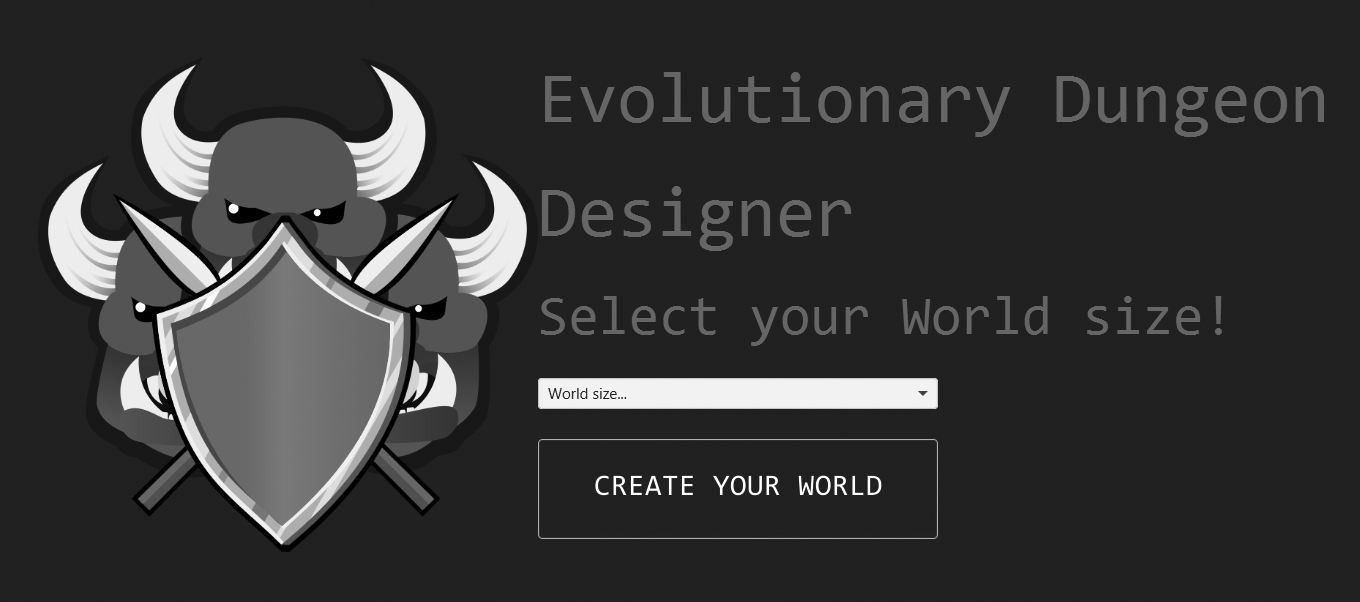
\includegraphics[width=1\columnwidth]{included-papers-tex/paper-1/figures-extra/start-edited.png}
    \caption{The start screen lets users choose the dungeon dimensions.}~\label{p1fig:launch}
\end{figure}

Previous research presented the \emph{Evolutionary Dungeon Designer} (EDD)~\citepone{p1Eddy1_5, p1Eddy2} as a mixed-initiative authoring tool for designing dungeon rooms for adventure games. EDD automatically generates and suggests rooms to the user while the user is manually designing one of them. The user either form the room from scratch or from a previously generated suggestion. This is done by means of a FI-2Pop GA~\citepone{p1kimbrough_feasibleinfeasible_2008}, where game design patterns are used both as input parameters and as objectives. These patterns involve micro-patterns (\textsc{Enemy}, \textsc{Treasure}, \textsc{Chamber}, \textsc{Corridor}, \textsc{Connector}, \textsc{Entrance}, and \textsc{Door}) as well as meso-patterns (\textsc{Ambush}, \textsc{Guard Chamber}, \textsc{Treasure Chamber}, and \textsc{Guarded Treasure}). EDD also ensures that all generated rooms are playable.

Initial experiments on EDD~\citepone{p1Eddy1_5} validated its PCG system in terms of fitness optimization, pattern detection, and solution diversity, providing a sufficient level of control to the designer. The following iteration~\citepone{p1Eddy2} explored the capabilities of EDD as a mixed-initiative level generator as a means of facilitating collaboration between human designers and PCG algorithms. Among its key features, the participants of a user study highlighted EDD as a useful framework for working with game design patterns in the context of search-based problems. The suggestions were considered a good source of inspiration as well as time saving. This user study also shaped the roadmap for future improvements on EDD. This included extending EDD from room generation to complete dungeon generation, and preserving the users' designs to a higher degree in relation to both design patterns and room aesthetics.

This version of EDD extends previous work based on the aforementioned user study by implementing the following key improvements:

\begin{itemize}
  \item The designer is now able to construct, develop, and edit a grid-based dungeon of different dimensions and inter-connected rooms, in contrast to a single room, which in turn, helps the designer on having context over their work on individual rooms and giving them more freedom on producing variations.
  \item The designer receives extended information about the consequences of their changes in individual rooms, and the differences between the current edited room and the proposed suggestions by the EA.
  \item The UI has been renovated to account for the newly added features by means of different views and options, as well as, a better structure and distribution of the different elements in the generator.
  \item Navigation tools have been added within a view and between views, which provides an overview of the dungeon, along with a better context of the edited room.
  \item The EA has been updated to assess and preserve the aesthetic criteria of the designer by means of a new capability of locking sections of an edited room for preserving custom aesthetic structures, and by extending the evaluation function through the measurement of symmetry and similarity in the provided suggestions, both which are further explained in \citepone{p1Eddy2_5}.
\end{itemize}

\subsection{Improving the Mixed-Initiative Evolutionary Dungeon Designer} \label{p1approach}

\cref{p1fig:launch} shows the start screen in EDD, which starts a new workflow by prompting users to choose the maximum number of rooms in the dungeon to be developed. The dimensions range from 2x2 rooms up to 7x7 rooms in a square dungeon grid (also referred as world grid). From this point, the workflow offers users three different views: 1) a world view for dealing with aspects regarding the dungeon as a whole; 2) a room view which places the focus in a particular room in the dungeon; and 3) the suggestions view, which produces six different suggestions with diverging room configurations (e.g. more corridors or more chambers) for the user to choose from. The user can freely alternate between views during the design process. The current dungeon layout can be saved at any moment from either of the views.

\begin{figure}[t]
    \centering
    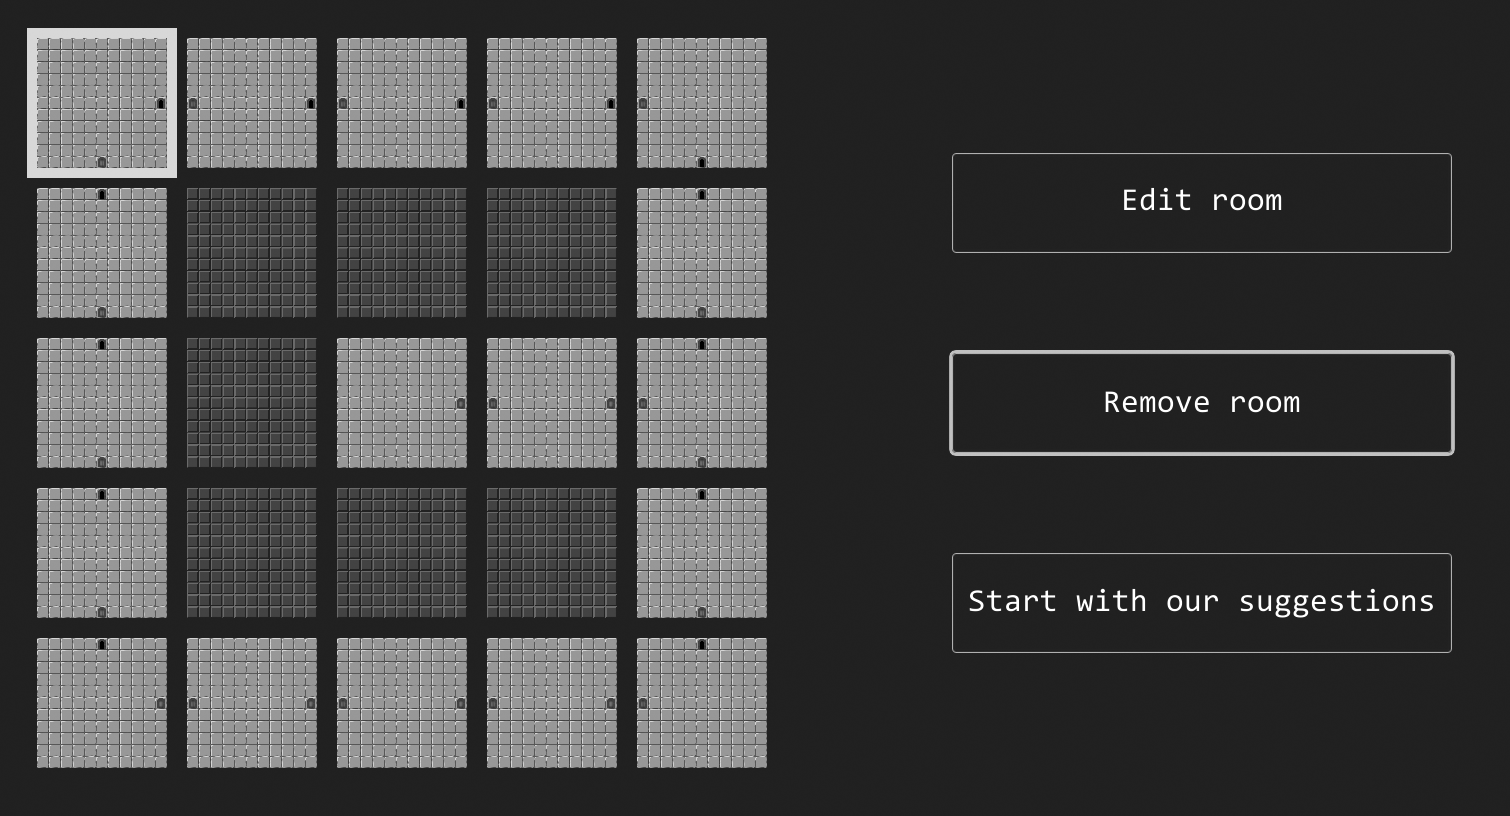
\includegraphics[width=\columnwidth]{included-papers-tex/paper-1/figures-extra/world-edited.png}
    \caption{Sample world view showing a 5x5 dungeon with 7 disabled rooms. User actions are displayed in the rightmost buttons.}~\label{p1fig:world}
\end{figure}

The world view (\cref{p1fig:world}) opens up right after the start screen, displaying a grid of the selected size composed by a fully connected set of empty rooms (all rooms are connected to their neighbors). The users can load a previously saved dungeon design, skipping the start screen and resume work from the state in which the dungeon design was saved.

From the world view users can then click and select any room to:
\begin{itemize}
\item disable or enable the room. Disabling makes the room inaccessible, removing all doors from the adjacent rooms. This can be undone by clicking \emph{enable}. Single rooms that become isolated after all their neighbors have been disabled, are automatically disabled as well. \cref{p1fig:dungeon1,p1fig:dungeon2} show two examples of dungeons with several disabled rooms,
\item get procedurally generated suggestions for that room in the suggestions view,
\item load the room in the room view for manual editing.
\end{itemize}

\begin{figure}[!ht]
    \centering
     \subfloat[\label{p1fig:dungeon1}]{%
       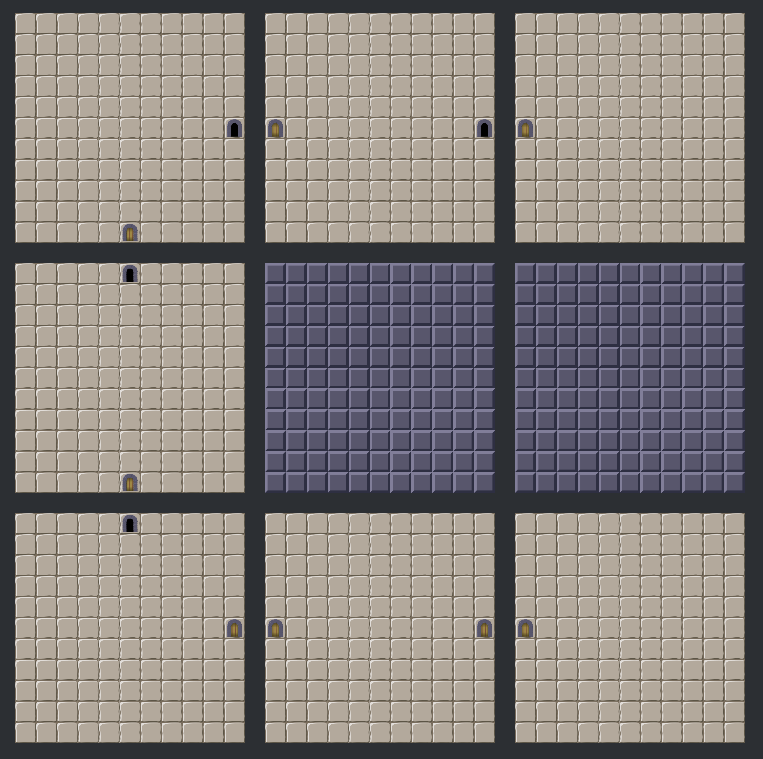
\includegraphics[width=0.49\textwidth]{included-papers-tex/paper-1/pap1-Figures/dungeon1.png}
     }
     \hfill
     \subfloat[\label{p1fig:dungeon2}]{%
       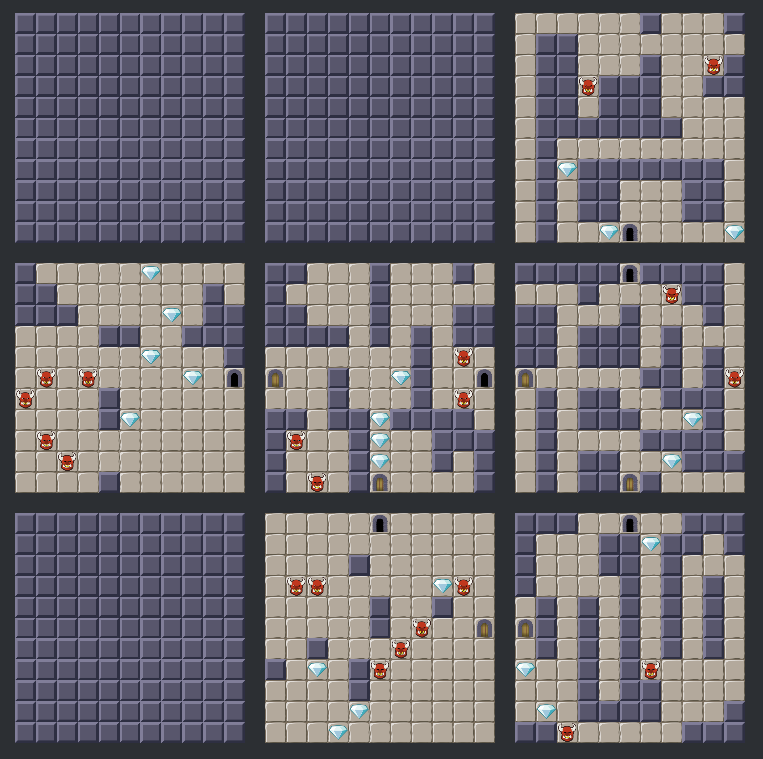
\includegraphics[width=0.49\textwidth]{included-papers-tex/paper-1/pap1-Figures/dungeon3-edited.png}
     }
    
    \caption{(a) 3x3 dungeon with 2 disabled rooms and 7 empty rooms, and (b) 3x3 dungeon completed dungeon with 3 disabled rooms.}
    \label{p1fig:dungeonsp1}
\end{figure}

\subsubsection{The Suggestions View}

By selecting ``Start with our suggestions'' in the world view (\cref{p1fig:world}) six uniquely generated rooms are presented to the user in a separate window: the suggestions view (\cref{p1fig:suggestionsview}). When clicking any of the suggestions, it will replace the previously selected room in the dungeon.

\begin{figure}[!ht]
    \centering
    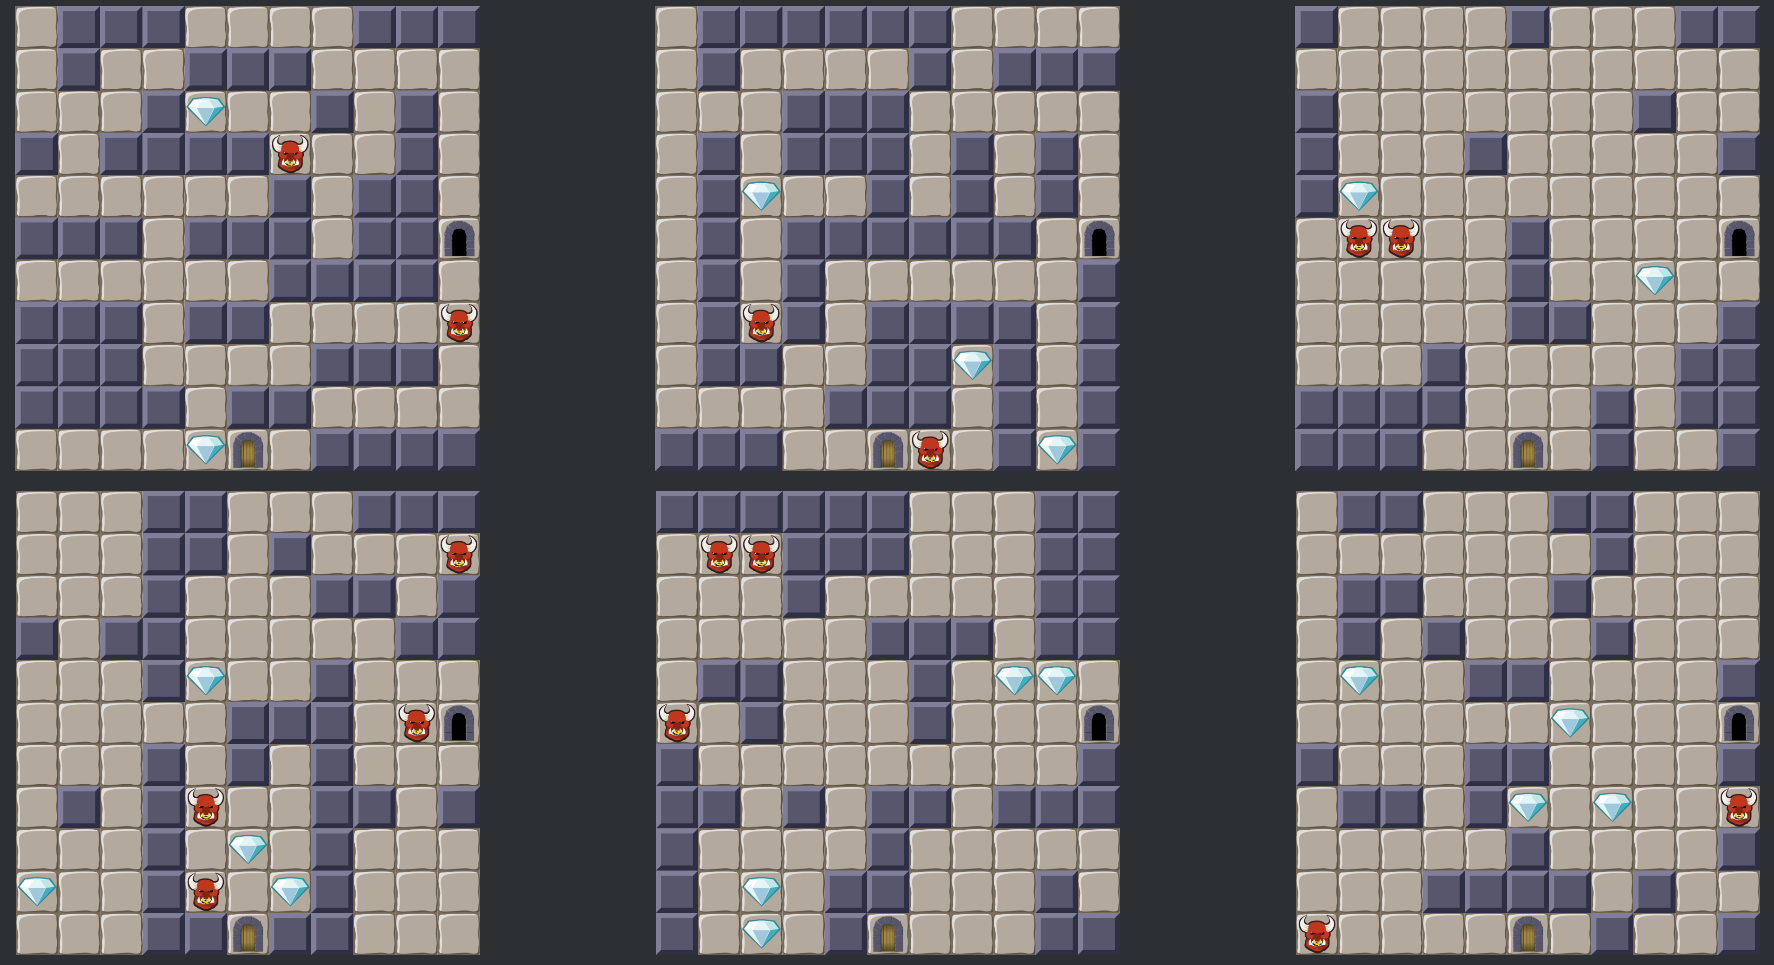
\includegraphics[width=\columnwidth]{included-papers-tex/paper-1/pap1-Figures/suggestionsview.png}
    \caption{Six procedurally generated rooms presented to the user in the suggestions view.}~\label{p1fig:suggestionsview}
\end{figure}

A similar functionality was present in the former version of the tool, presented only once as the start screen. Now users can freely alternate between the world and the suggestions views, getting as many suggestions as they need, deciding whether to start creating every room from a clean state or to get inspiration from one of the generated rooms.

\begin{figure*}[t]
    \centering
    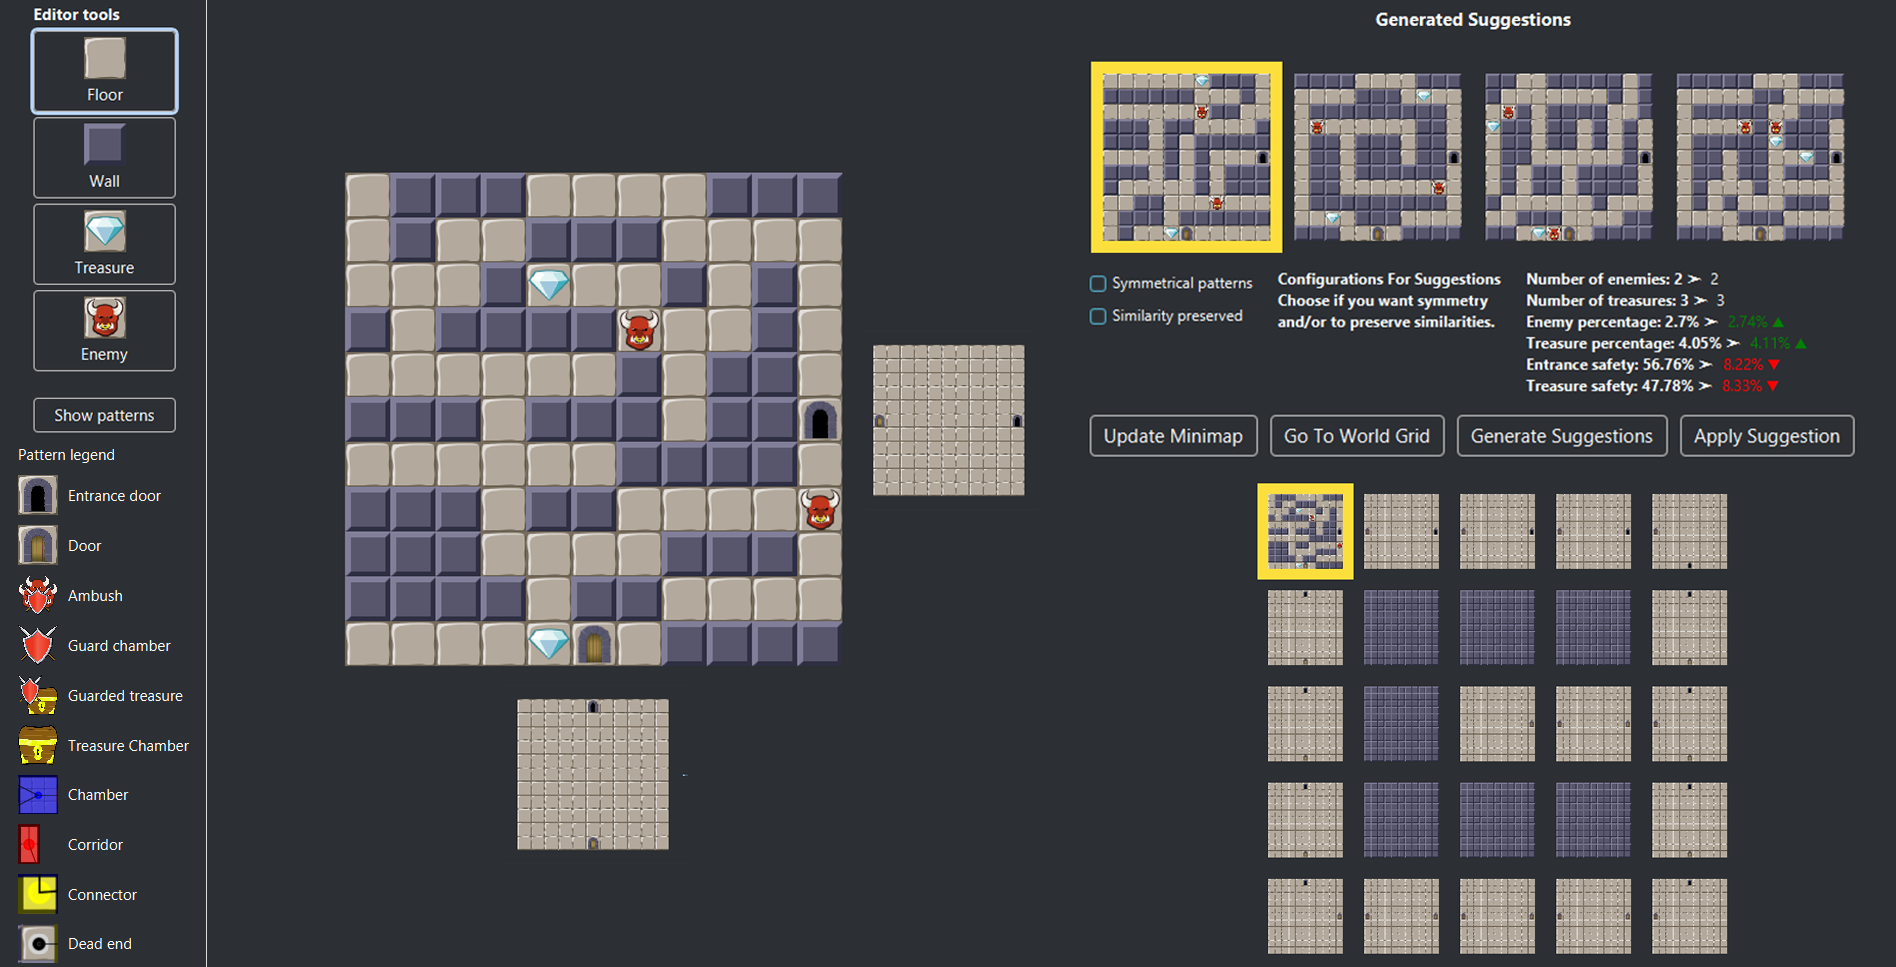
\includegraphics[width=\textwidth]{included-papers-tex/paper-1/pap1-Figures/roomview.png}
    \caption{The room view while editing the top-left corner in a 5x5 dungeon with seven disabled rooms.}~\label{p1fig:roomview}
\end{figure*}

Suggestions preserve the door layout from the room that was selected in the world view. The suggestions shown in \cref{p1fig:suggestionsview} have been created for the room selected in \cref{p1fig:world}, placed in the top-left corner, and containing only two doors connecting them to their east and south neighbor.

\subsubsection{The Room View}

\begin{table*}[ht]
% \centering
\caption{General consensus on EDD's features} \label{p1tab:consensus}
\resizebox{0.8\textwidth}{!}{
\begin{tabularx}{\textwidth}{|p{0.2\textwidth}|p{0.99\textwidth}|}
\cline{1-2}

Description & Participants’ Consensus \\\cline{1-2}
World Grid  of the dungeon                   & Its purpose of establishing an illusion of a fully realized dungeon is somewhat achieved. However, limitations exist with how it defines feasibility, a dungeon’s starting point, and the entrances, which disrupts the designers’ decisions.                                                                                                                                                                                   \\\cline{1-2}
World View                                  & The world view’s usefulness for the most part could not be established, other than for the purpose of going to the suggestions view (which was already seldom during the user study) and having a closer look at the entire dungeon without any distractions. Some participants preferred features to be already in the room view’s minimap, and some wanted to see more specific functionalities within the world view itself. \\\cline{1-2}

Enabling and  \newline disabling rooms                & As the user study restricted participants to create 3x3 dungeons, this feature for the most part has been neglected. This is also in part because of its accessibility only being in the world view, which proved to be an inefficient view in general. However, its use for bigger dungeon sizes later on was appreciated, especially for more intricate design purposes.                                                      \\\cline{1-2}
Suggestions View                            & Similarly to enabling and disabling rooms, it was quite difficult to encourage the use of this functionality due to the world view’s inefficient usability. However, this could also be due to the dungeon’s small size, as some participants expressed high interest in using more suggestions with larger dungeon sizes.                                                                                                      \\\cline{1-2}
Minimap  \newline  navigation                      & The minimap proved to be a strong tool not only for navigation purposes, but also for supporting design decisions and choices. The directional buttons were rarely used, but their room previews were helpful in emphasizing the current room’s connection to adjacent rooms without looking at the minimap. On the other hand, this lowered the usability of the world view.                                                   \\\cline{1-2}
Parameters                                       & The parameters were, in general, lacking. They served to be important in decision-making when choosing a suggested map in room view, but there were still doubts on their accuracy and sufficiency when providing information about the generated suggestions.                                                                                                                                                                       \\\cline{1-2}
Generated maps for  \newline  suggestions in room view & Suggestions in the room view proved to be very helpful in supporting the whole design process as they primarily acted as inspirations for the users. The most prominent comment among the users is the preference of having more control on how suggestions should be generated depending on different types of parameters.                                                                                                     \\\cline{1-2}
Design \newline  patterns& The patterns’ visualization was, in general, lacking and not self-explanatory. Some participants have expressed interest in using patterns as a parameter in the generation of suggestions.                                                                                                                                                                                                                                     \\\cline{1-2}
Dark theme                                  & EDD’s dark theme for the user interface received a positive response as it makes working with the program easier.
	\\ \cline{1-2}
\end{tabularx}
}
\end{table*}

% \begin{table}
% \begin{center}
% {\caption{Best performing setups based on their internal validation and visualization of clustered data points.}\label{table:setups}}
% \resizebox{\textwidth}{!}{
% \begin{tabular}{ccccccc}
% \hline
% \rule{0pt}{12pt}
% Algorithm&Data&K&$\Diamond$&$\Box$&$\bigtriangleup$ 
% \\ 
% \hline
% \\[-6pt]
% K-Means & Tiles-PCA & 9 & 0.43 & 0.73 & 9438.233 \\ 
% K-Means & Tiles-PCA & 12 & 0.41 & 0.77 & 9436.928 \\
% K-Means & Dimensions-PCA & 12 & 0.43 & 0.73 & 7738.343 \\
% Agglomerative single & Combined-PCA & 6 & 0.51 & 0.43  & 38.833 \\ 
% Agglomerative avg. & Dimensions-PCA & 6 & 0.44 & 0.67 & 3463.567 \\ 
% \hline
% \\[-6pt]
% \multicolumn{6}{l}{$\Diamond$ Silhouette Score\ \
% $\Box$ Davies Bouldin Index\ \
% $\bigtriangleup$ Calinski-Harabasz Index}
% \end{tabular}
% }\end{center}
% \end{table}

Users edit single rooms in the room view (\cref{p1fig:roomview}), regardless of whether these are new empty rooms, procedurally generated suggestions, or previously edited rooms. The room view is an improved and extended version of the main screen in the last version of EDD~\citepone{p1Eddy2}. All functionalities from that version are still present: manually editing the room by changing tiles (floor, wall, enemy, and treasure), displaying an overlay view of the existing design patterns, and procedurally generating suggestions based on the current edited room's configuration.

Navigation is one of the crucial added features, allowing users to move around the dungeon without going back to the world view. Two other options offer navigation through the dungeon: the navigational buttons and the minimap. The navigational buttons are displayed next to each of the edited rooms' borders that contain a door. Provided that the room being edited in \cref{p1fig:roomview} is located in the top-left corner, two navigational buttons are displayed right and below the room, respectively. Clicking a navigational button transports the user to that room, replacing the currently edited room with the targeted neighbor. Instead of using arrows or any other fixed picture, these buttons preview the neighboring rooms as a hint for users to help them design the room currently being edited. The navigational buttons are automatically refreshed to reflect up-to-date changes performed to the neighboring rooms.  

The minimap displays a scaled-down overall picture of the whole dungeon, highlighting the currently edited room with a yellow border. Users can navigate to any room, which is not disabled and is displayed on the minimap by clicking on it, replacing the current room. The buttons above the minimap allow users to go \textit{Back To World Grid}, to \textit{Update Minimap}, as well as request and select procedurally generated suggestions. The whole minimap is updated whenever the user navigates to a different room, but if the user wants to see the last changes applied to currently edited room reflected on the minimap, a manual refresh has to be done. This is done to reduce the workload derived from re-rendering the minimap automatically after every manual edition.

The generated suggestions work similarly to the previous version of EDD: four unique maps are generated by the underlying evolutionary algorithm in four subsequent evolutions, seeding the four initial populations with different sets of features extracted from the edited room. Each suggestion is evolved by means of a different fitness function, therefore addressing different goals to maximize diversity in the provided suggestions. Clicking on a suggestion highlights it, and clicking \textit{Apply Suggestion} replaces the current room with the highlighted map. This differs from the previous version, in which maps were applied at the moment they were clicked on, occasionally causing work loss due to accidental replacements. 

Additionally, highlighted suggestions display informative parameters below them. These describe meaningful features of the highlighted room that are relevant to both the human designer and the evolutionary algorithm's fitness calculation: number of enemies and treasures, enemy and treasure rate (in relation to floor tiles), and entrance and treasure safety (see \citepone{p1Eddy1_5} for a detailed description). These parameters are displayed as a comparison between their values in the edited room and in the highlighted suggestion, showing how they would change if the suggestion is applied. 

Two checkboxes below the suggestions now offer users the possibility to ask specifically for the provided suggestions to address symmetry and similarity aesthetic features, respectively. By ticking the symmetry checkbox, two of the suggestions will be generated by the evolutionary algorithm using a symmetry fitness function, which enable the generation of symmetric rooms, (either vertically, horizontally, or diagonally). Analogously, ticking the similarity checkbox, the other two suggestions are generated with a similarity fitness function, which promotes the generation of room aesthetically similar (but never equal) to the currently edited map. These fitness functions are presented in~\citepone{p1Eddy2_5}. When both checkboxes are unchecked, the fitness functions described in~\citepone{p1Eddy2} are used.

\subsection{User Study} \label{p1userstudy} 

\begin{table}[ht]
% \centering
\caption{Participants’ most requested features} \label{p1tab:demands}
% \resizebox{\paperwidth}{!}{\begin{minipage}{\paperwidth}
\resizebox{0.8\textwidth}{!}{
% \begin{tabularx}{\textwidth}{|p{0.2\textwidth}|p{0.99\textwidth}|}
\begin{tabularx}{\textwidth}{|p{0.2\textwidth}|p{0.99\textwidth}|}
\cline{1-2}
Feature                                 & Description                                                                                                                                                                                                                                                                                                                                                                                                         \\\cline{1-2}
Design patterns                   & Their visualization and accuracy should be improved. Other than acting as visual guide for map information, they should be used to help generate rooms as well. They should also be available for the entire dungeon.                                                                                                                                                                                 \\\cline{1-2}
Parameters                                  & They need to have more information about the specific room, and have better visualization in order to make the designer trust their accuracy more. The parameters should also consider the entire dungeon as a whole in different terms such as difficulty and balance.
\\\cline{1-2}
Generated suggestions               & In general, the participants want more variety and control in the generation of suggestions using different types of parameters e.g. their degree of similarity and fitness functions.                                                       \\\cline{1-2}
Redefined feasibility                           & Eddy 3.0’s definition of feasibility should be revised which considers the whole dungeon and its connected rooms.                                                                                                      \\\cline{1-2}
World View                      & The World View should be revised and enhanced with more special features which would encourage users to visit it more.                                                    \\\cline{1-2}
World grid                                       & The computation of the whole dungeon should be improved. It should have an option to define a starting point. Its definition of entrance doors should be improved, as well as the calculation of distances of tile types.                                                                                                                                                                       \\\cline{1-2}
Version control & Some participants want to preview suggestions within the Room View to help their judgment and the ability to save suggestions for later use. They also want to revert to old designs in case they have second thoughts.                                                                                                     \\\cline{1-2}
Templates                             & Some participants want the ability to save their own manual designs to be carried over to other grids.                                                                                                                                                                                                                                     \\\cline{1-2}
Automated assistance                                  & The participants in general welcome a bit more automated assistance when doing manual designs, which can reduce clicking around the program. It should also not be too invasive for the designer. 
	\\ \cline{1-2}
\end{tabularx}
}
% \end{minipage}}
\end{table}

% \begin{table}[h]
% \centering
% \caption{Developed game based features used as dimensions in the~\acrlong{icmape}}\label{table:mape-dimensions}
% % \resizebox{\textwidth}
% % \resizebox{\textwidth}
% \begin{tabularx}{\textwidth}{|c|X|}
% \cline{1-2}
% \rule{0pt}{12pt}
% Feature&Definition\\ \cline{1-2}
% % \\[-6pt]
% Similarity & Refers to the aesthetic (tile-by-tile) similarity between a room and the current designer's design.\\ \cline{1-2}
% Inner Similarity & Refers to the similarity of the sparsity and density of the different tile types of a room designer's current design.\\ \cline{1-2}
% Symmetry & Refers to the aesthetic symmetry of a room.\\ \cline{1-2}
% Leniency & Refers to how challenging rooms are; calculated based on the position of enemies and balance between enemies and treasures.\\ \cline{1-2}
% Linearity & Refers to the amount of paths connecting doors within a room; calculated based on how many spatial patterns are traversed.\\ \cline{1-2}
% \#Meso-Patterns & Refers to the number of meso-patterns that exist within a room, normalized by an estimated maximum number based on the room's size and the minimum chamber size.\\ \cline{1-2}
% \#Spatial-Patterns & Refers to the number of spatial-patterns that exist within a room, which can be chambers, corridor, turns, junctions, and intersections.\\ \cline{1-2}
% \end{tabularx}
% \end{table}

A user study was conducted in order to assess the impact on the design process caused by the improvements made to EDD. Five game developers participated in the study, which had the following structure:
\begin{itemize}
\item \textit{Introduction to the purpose of the study}. Participants were asked whether they were familiar with the previous version of EDD.
\item \textit{Demonstration of the tool}, showcasing its workflow and features with a short example performed over a 3x3 dungeon. 
\item \textit{Designing a dungeon}. After the demonstration the users were tasked to design a 3x3 dungeon within approximately 10 minutes, saving the work after that for a later analysis and discussion conducted in a structured interview with the participant after this phase. Two observers took notes of what the participant was doing, providing additional data for the later analysis.
\item \textit{Questionnaire}. The users were asked a few questions regarding their background in game design as well as dungeon-based games. They were also asked whether they had any previous experience with mixed-initiative tools.
\item \textit{Interview}. A semi-structured interview was conducted to provide data for an analysis and discussion about the tool, and its improvements. Audio was recorded for a later analysis.
\end{itemize}

As as result of the questionnaire, the following information was gathered from the participants:
\begin{itemize}
\item User 1 has been working for more than ten years in the game industry as a data scientist and user experience researcher. The user holds prior experience with RPGs and dungeon crawlers, and is familiar with the terms of mixed-initiative tools and has used The Sentient Sketchbook in the past. This user is the only one who participated in the former user study of EDD.
\item User 2 has been working for six months as a project coordinator of eSports events and has long experience of playing dungeon crawlers and RPGs. This user is not familiar with mixed-initiative concepts and has never used a mixed-initiative authoring tool before.
\item User 3 has been working for six years in the game industry as a user experience researcher and a biometrics expert. The user has prior experience with dungeon style games, but has limited knowledge about mixed-initiative tools.
\item User 4 has been working for nine years as a senior user experience researcher and has long experience of playing dungeon crawlers and RPGs. This user is not familiar with mixed-initiative concepts and has never used a mixed-initiative authoring tool before. 
\item User 5 has been working for three weeks as a game user researcher. This user has no experience with dungeon crawlers and dungeon-based RPGs, and is not familiar with mixed-initiative tools. 
\end{itemize}

\subsection{Results and Discussion} \label{p1conclusion} 

As with any raw qualitative data, the data collected from the user study has to go through a condensation process in order to isolate the most relevant information that will answer the research questions. In a blueprint provided by~\citepone{p1srnka2007words}, the qualitative data obtained has undergone four out of five stages: 
\begin{itemize}
\item \textit{Material sourcing}: an audio recording the user study, interview materials, and the authors’ own observations.
\item \textit{Transcription}: combining and writing down the observations and questionnaire answers for each participant in the user study.
\item \textit{Unitization}: dividing the data according to the mixed-initiative features of EDD.
\item \textit{Categorization}: dividing the data according to categories relevant to the research questions while taking into consideration the principles of mixed-initiative.
\end{itemize}

All participants in the user study perceived EDD as overall good and intuitive. \cref{p1tab:consensus} shows their general consensus of EDD's usability and capability to foster creativity in dungeon design. \cref{p1tab:demands} lists the participants' most requested missing features.

The main goal of mixed-initiative interaction pertains to the flexibility of roles between the human and computer as a team and simplifying the general experience~\citepone{p1allen1999mixed}, and this was somewhat achieved by EDD. This could be proven by how features such as suggestions and the implementation of a whole dungeon with navigation have definitely supported the users when making decisions throughout the design process. As a result the experience was overall simple and intuitive. It could not be said, however, that the set goal has been fully achieved; a fully successful mixed-initiative system emphasizes interchangeable roles of the human and computer while maintaining the balance between them. The participants in the user study did not feel restricted, but they still desired more control in EDD’s assistance in the design process, as well as different suggestions that the designer cannot come up with themselves.

\citepone{p1horvitz1999principles} provides a list of principles for mixed-initiative user interfaces which would enhance human-computer interaction. EDD has achieved four out of twelve in Horvitz’s list of critical factors that would make up a fully successful mixed-initiative system:

\begin{itemize}
\item \textit{Developing significant value-added automation}: providing an automated solution that cannot be achieved with direct manipulation. EDD provides a framework for the generation of complex dungeons of different sizes, together with suggestions of similar dungeon rooms and information parameters for these suggestions. 
\item \textit{Considering uncertainty about a user’s goals}: taking advantage of a user’s uncertainty in their intentions. EDD provides the choice to initialize rooms in a dungeon with either an empty slate or from any of the generated suggestions.
\item \textit{Inferring ideal action in light of costs, benefits, and uncertainties}: considering the value of an automated service in regards to the usually expected value of taking actions. EDD’s main motivation is to significantly reduce the cost of game design while maintaining and improving creativity, which has at least partially been fulfilled.
\item \textit{Employing dialogue to resolve key uncertainties}: establishing an efficient dialog between the human and computer when uncertainty arises while considering the costs of potentially disrupting the user. EDD extracts and displays relevant features in the edited and suggested rooms for the users to guide their decisions. The minimap also fulfill parts of this role.
\end{itemize}

There are other principles which are relevant to EDD which fall in line with the participants’ feedback. For example, some principles such as the ability to continuously learn from the user’s input and to preserve memory of their decisions and actions may pertain to the desired features of having more control in the generation maps and receiving more assistance in preserving their own manual designs for different purposes.

\subsection{Conclusions and Future Work}

The contributions presented in this work explore how the user interface and the mixed-initiative aspects in the Evolutionary Dungeon Designer have been improved, as well as how they should be improved on further in order to increase creativity during the dungeon design process.

The addition of the world grid provides the adoption of a new workflow, which offers users the possibility to start designing either from empty rooms or PCG suggestions. Various changes in the user interface were made to accommodate the increased dungeon size. With a larger dungeon, navigation has proved to be a key functionality, as well as giving an overview of the adjacent rooms. Now users can get a better understanding of the context of the room currently being edited. In conjunction with the navigation and larger dungeons, a minimap was also added to further enhance the experience when designing a larger dungeon. Alongside these changes, aesthetic goals have been included in the generative process. Visual cues for room descriptors were added, so that the user can make a more informed decision when selecting suggested maps.

Compared to its previous version, EDD further empowers the mixed-initiative design process by providing more context, feedback, flexibility, and to some extent, the ability to address aesthetic features in the procedural suggestions. Creativity can directly adhere to the amount of interesting possibilities a designer can employ, which is relevant to providing rich contexts to dungeon designs. EDD offers a mixed-initiative experience that provides adequate flexibility for the designer’s intentions as the results from the user study have shown.

Overall, our user study successfully shows the strengths of mixed-initiative tools for designers but it also reveals various limitations, which should be considered by the community when creating a mixed-initiative tool.

To a certain extent, controllability is preferred than expressivity, as the users continuously try to impose their vision, which is a non-trivial task for automated systems to capture, thus, the users are more likely to sacrifice to a certain degree expressivity and exploration of the tool by gaining control over the generated content. 

The capability of proposing useful and novel suggestions is fundamental to fostering creativity and impulses the generation of more interesting content. Moreover, explicit information about the designers’ changes and choices is important as it helps them understand the effect of their decisions. 

Finally, this work has identified features that should still be taken into consideration for future versions of the tool, which are shown in \cref{p1tab:demands}.

\subsection*{ACKNOWLEDGMENTS}
The Evolutionary Dungeon Designer is part of the project \textit{The Evolutionary World Designer} which is supported by The Crafoord Foundation.

% \let\oldthebibliography=\thebibliography
% \renewenvironment{thebibliography}[1]{%
%   \oldthebibliography{#1}%
%   \setcounter{enumiv}{0}%
% }

% \bibliographystyle{ieeetr}
\bibliographystylepone{ieeetr}
% \phantomsection
% \addcontentsline{toc}{section}{REFERENCES}
\bibliographypone{included-papers-tex/paper-1/references}